\documentclass[ fontsize=11pt]{article}
\linespread{1.5}
% \usepackage[margin=2.5cm]{geometry}
\usepackage[margin=2.5cm, headheight=0pt, headsep=1cm]{geometry}
\usepackage{enumerate, fancyhdr, graphicx, amsmath, float}
\usepackage{hyperref}


\title{Old School \tetris{} Meets Page Rank}
\author{Paul Chesnais (pmc85) \& Sam "Sven" Svenningsen (sjs382)}
\date{}

\def\tetris{Tetris\textsuperscript{\textregistered}}

\pagestyle{fancy}
\fancyhead{}
\lhead{pmc85 \& sjs382}
\chead{Old School \tetris{} Meets Machine Learning}
\rhead{\today}
\fancyfoot{}
\rfoot{\thepage}
\lfoot{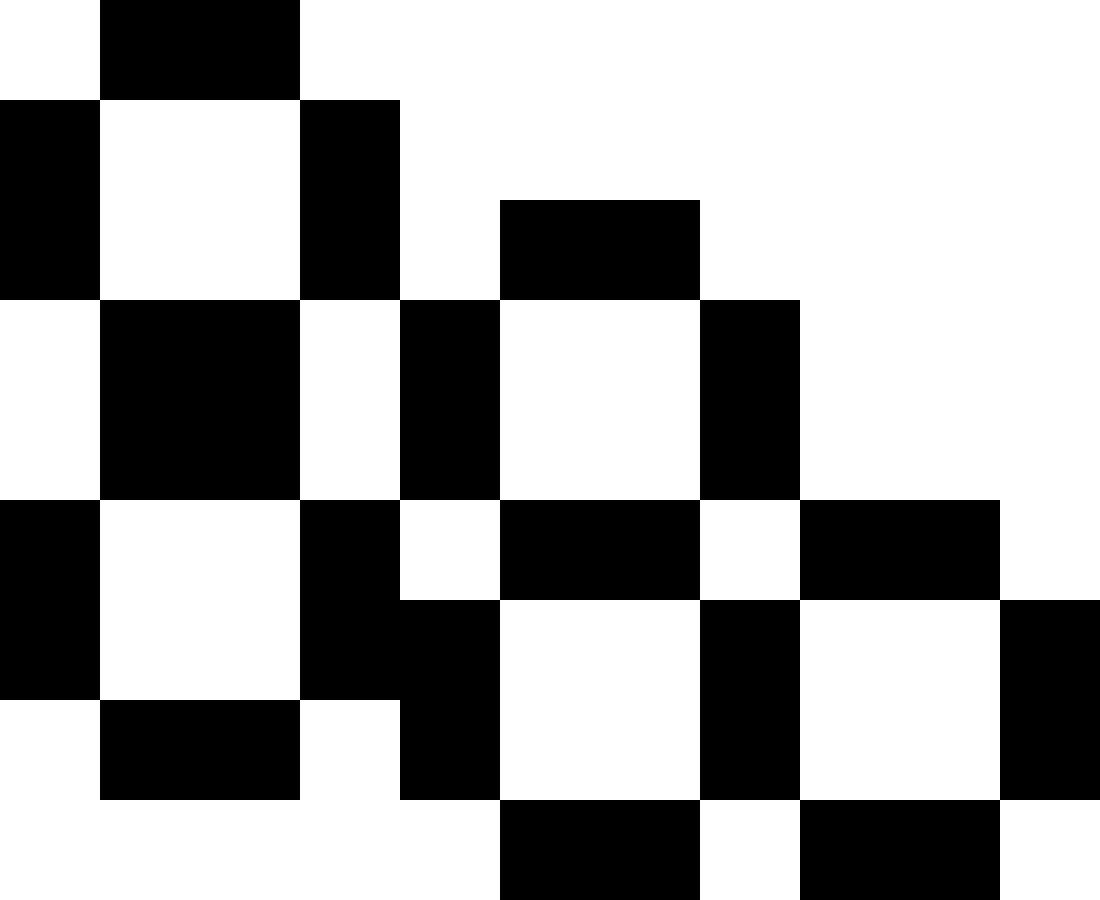
\includegraphics[height=20pt]{Logo}}
\renewcommand{\headrulewidth}{0.5pt}
\renewcommand{\footrulewidth}{0.5pt}


\begin{document}
\maketitle
\thispagestyle{empty}
\begin{figure}[H]
  \centering
  
\includegraphics[height=125pt]{tetris}
  \caption{The \tetris{} Logo}
  \label{fig:the_tetris}
\end{figure}
\begin{figure}[H]
  \centering
  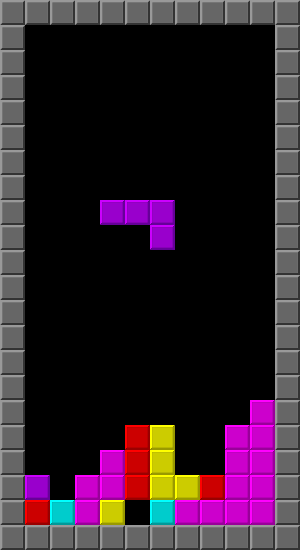
\includegraphics[height=300pt]{tetris_screen}
  \caption{A \tetris{} game in action}
  \label{fig:the_tetris_board}
\end{figure}
% \figure{\center{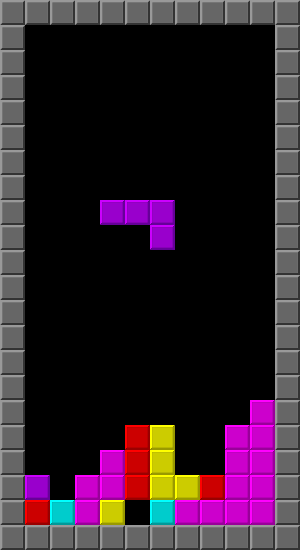
\includegraphics[height=300pt]{tetris_screen}}}
\newpage
\section{Abstract}
\label{sec:abstract}

\par We built a \tetris{} bot that plays \tetris{}, the Russian tile-matching puzzle video game. It has been shown that \tetris{} is NP-C \cite{tetrishard}, so none of our solutions are, or can be (assuming $P \neq NP$), perfect.  We solved it by simplifying the contour (of the top of the \tetris{} blocks on the board) into a sequence of incremental changes in height going left to right. Then we computed the rank of all possible contours iteratively, and ranked them. Then we used the PageRank algorithm to decide which pieces (and which orientations/locations) to go with. We also attempted a MiniMax solution, but were unable to complete it, but the attempt is discussed as well.




\section{Motivation}
\label{sec:motivation}
One of us is a super \tetris{}fan, and we thought it would be fun to make something that does well on a NP-Complete problem.


\section{Initial Attempts}
\label{sec:initial_attempts}

\subsection{MiniMax}
\par We tried to maximize the pieces placement in a way that would minimize the possible damage/maximize the least expected outcome of the next few pieces the \tetris{} board provides by using the MiniMax approach.
\subsubsection{Heuristic}
\par This lead us into the difficulty of grading boards on quality so that we could have a function to minimize over.

\par One thought would be to penalize boards that have holes or overhangs in them (i.e. pieces covering empty spaces), though penalize overhangs less since you can get around them sometimes.

\par The next obvious criteria was to give a max value to any board that has a \tetris{} (4 complete rows at once) and a lesser, but still high, score to any number of complete rows.

\par This leaves us an issue of all the boards with no obvious issues, and no obvious bonuses. We made a guess that having a more level board would be best (i.e. the distance between the lowest free spot and the highest tower you have is minimized).

\par An alternative to this is to make up as many features as possible and try to assign weights to them based on if they lead to failed games quickly (we'd have to play the game a bunch of times).

\par We weren't quite sure how to implement this though since we did not know how to weight each feature appropriately besides running it a million times over, which was too slow.

\subsubsection{Issues}
\par The size of the state space leads to some issues. There are about $10-40$ places to put a piece if you know which one it is (each piece has between 1 an 4 rotations and ~10 spots you can put it in), and $~190$ places you can put a piece each round for an unknown piece. So to do this n-places into the unknown piece space you have about $160*190^n$ pieces, which ends up being on the order of $10^{2n + 2}$ each round, even looking 4 pieces ahead into the unknown can take $10^{10}$ possible boards to check, which does not take a trivial amount of time.

\section{Challenges Faced}
\label{sec:challenges_faced}

\par Scala optimization


\section{Current Version}
\label{sec:current_version}



\section{Conclusion}
\label{sec:conclusion}

\newpage


\begin{thebibliography}{9}
\bibitem{tetrishard}
Erik D. Demaine, Susan Hohenberger, David Liben-Nowell
\textit{
Tetris is Hard, Even to Approximate}.
\\\href{https://arxiv.org/abs/cs/0210020}{arXiv:cs/0210020}

\end{thebibliography}


\end{document}
